\chapter{Идентификация системы связанных релаксационных генераторов}

\section{Реласкационные генераторы: применение, модели}

Применение: собственно генераторы, источники питания.

Элементная база, задачи. Почему возможны хаотические режимы

Не совсем прототип: Kennedy


\cite{mishenko_du_small_relax}

\section{Система из трёх связанных релаксационных генераторов на паре комплиментарных транзисторов}
\label{atu:sec:relax3d}

Основы

\begin{figure}[htb!]
  \centerline{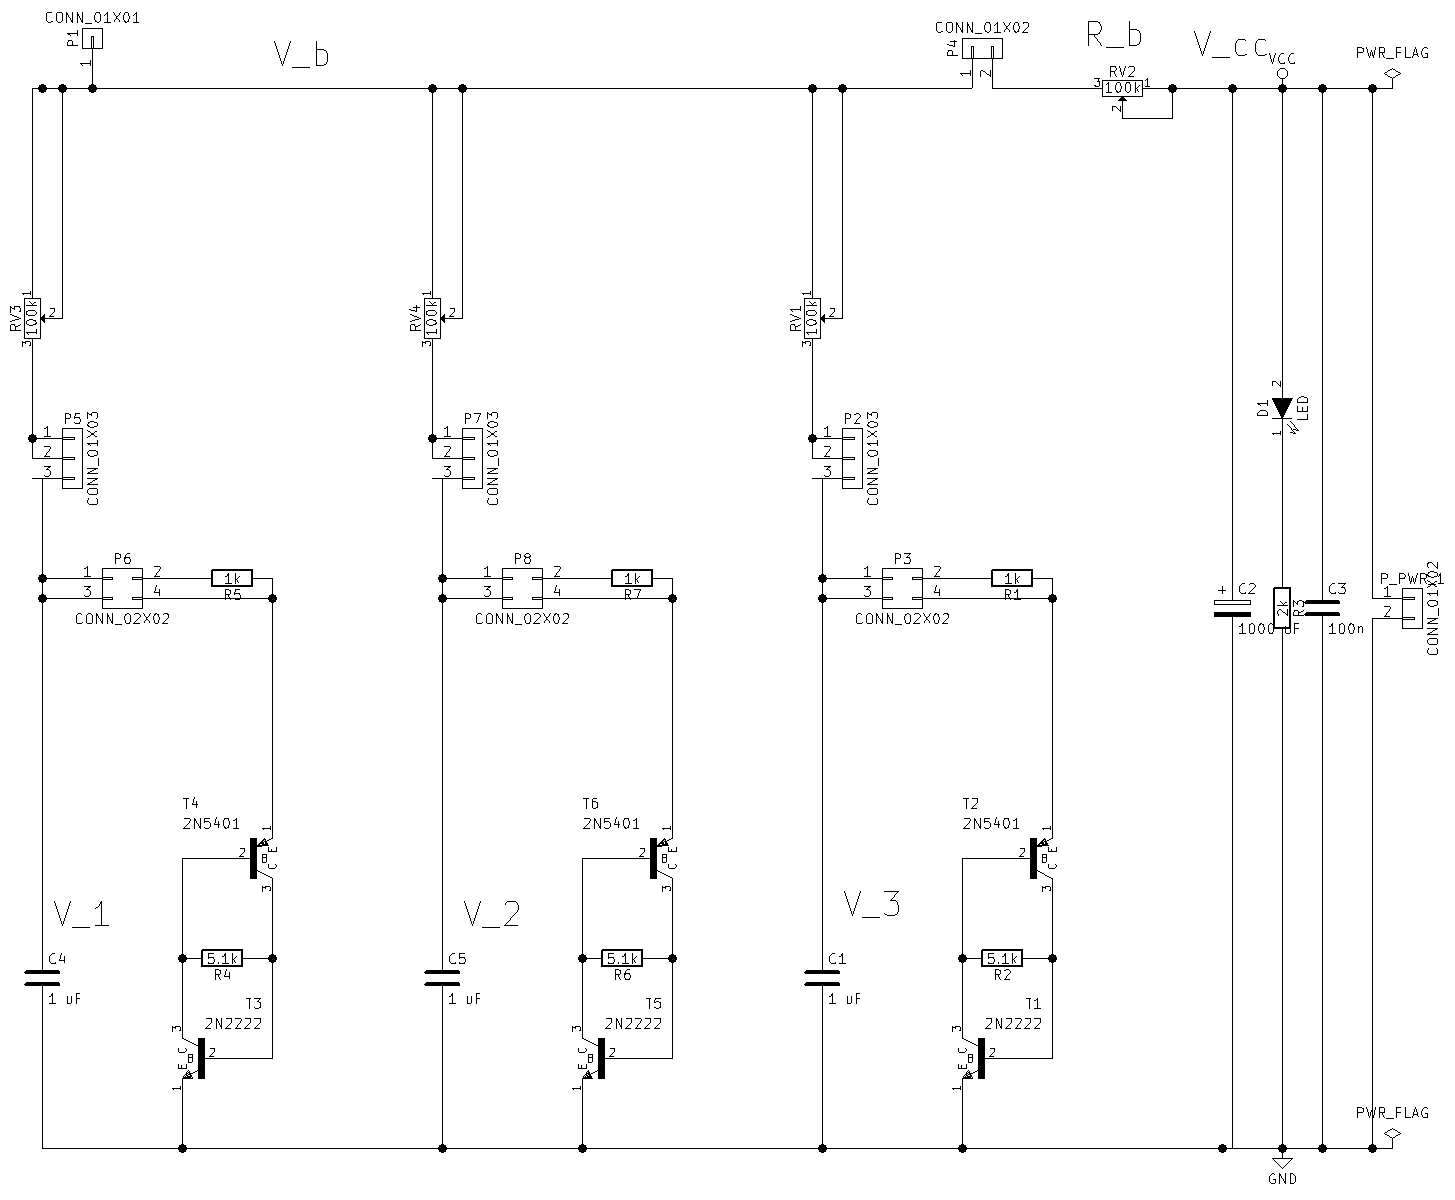
\includegraphics[width=0.7\textwidth]{p/relax3d_2bjt_schem.png} }
  \caption{Электрическая схема системы из трёх связанных релаксационных генераторов на паре комплиментарных транзисторов}
  \label{atu:relax3d_schem}
\end{figure}

Динамика.

\section{Система из трёх связанных релаксационных генераторов на основе триггеров Шмидта}
\label{atu:sec:relax3ds}

Схемотехническая реализация системы связанных релаксационных генераторов,
рассмотренная в разделе \ref{atu:sec:relax3d}, несмотря на ряд достоинств,
обладает определёнными недостатками. В первую очередь, следует отметить
тот факт, что при относительно высоких значениях величины $R_b$,
как раз при которых связь между отдельными генераторами становится существенной,
релаксационный элемент переключается из колебательного режима в режим
стабилизации напряжения, что не соответствует предназначению данной схемы.
Более того, в этих условиях зависимость тока от напряжения близка к экспоненциальной,
что затрудняет создание адекватной модели. При этом малые изменения параметров,
например, вызванные температурной нестабильностью, приводят к значительным изменением
тока, что также негативно сказывается на адекватности. Ещё один недостаток
заключается в том, что существующими элементами можно изменять напряжение срабатывания
в достаточно узком диапазоне, что затрудняет проведение как экспериментов,
так и моделирования в широком диапазоне параметров. В свою очередь,
это ставит вопросы о границах применимости модели, на которые сложно
ответить, опираясь на результаты эксперимента.

Таким образом, возникает задача синтеза схемы системы связанных
релаксационных генераторов, которая бы в минимальной степени была бы
подвержена вышеупомянутым недостаткам.



\begin{figure}[htb!]
  \centerline{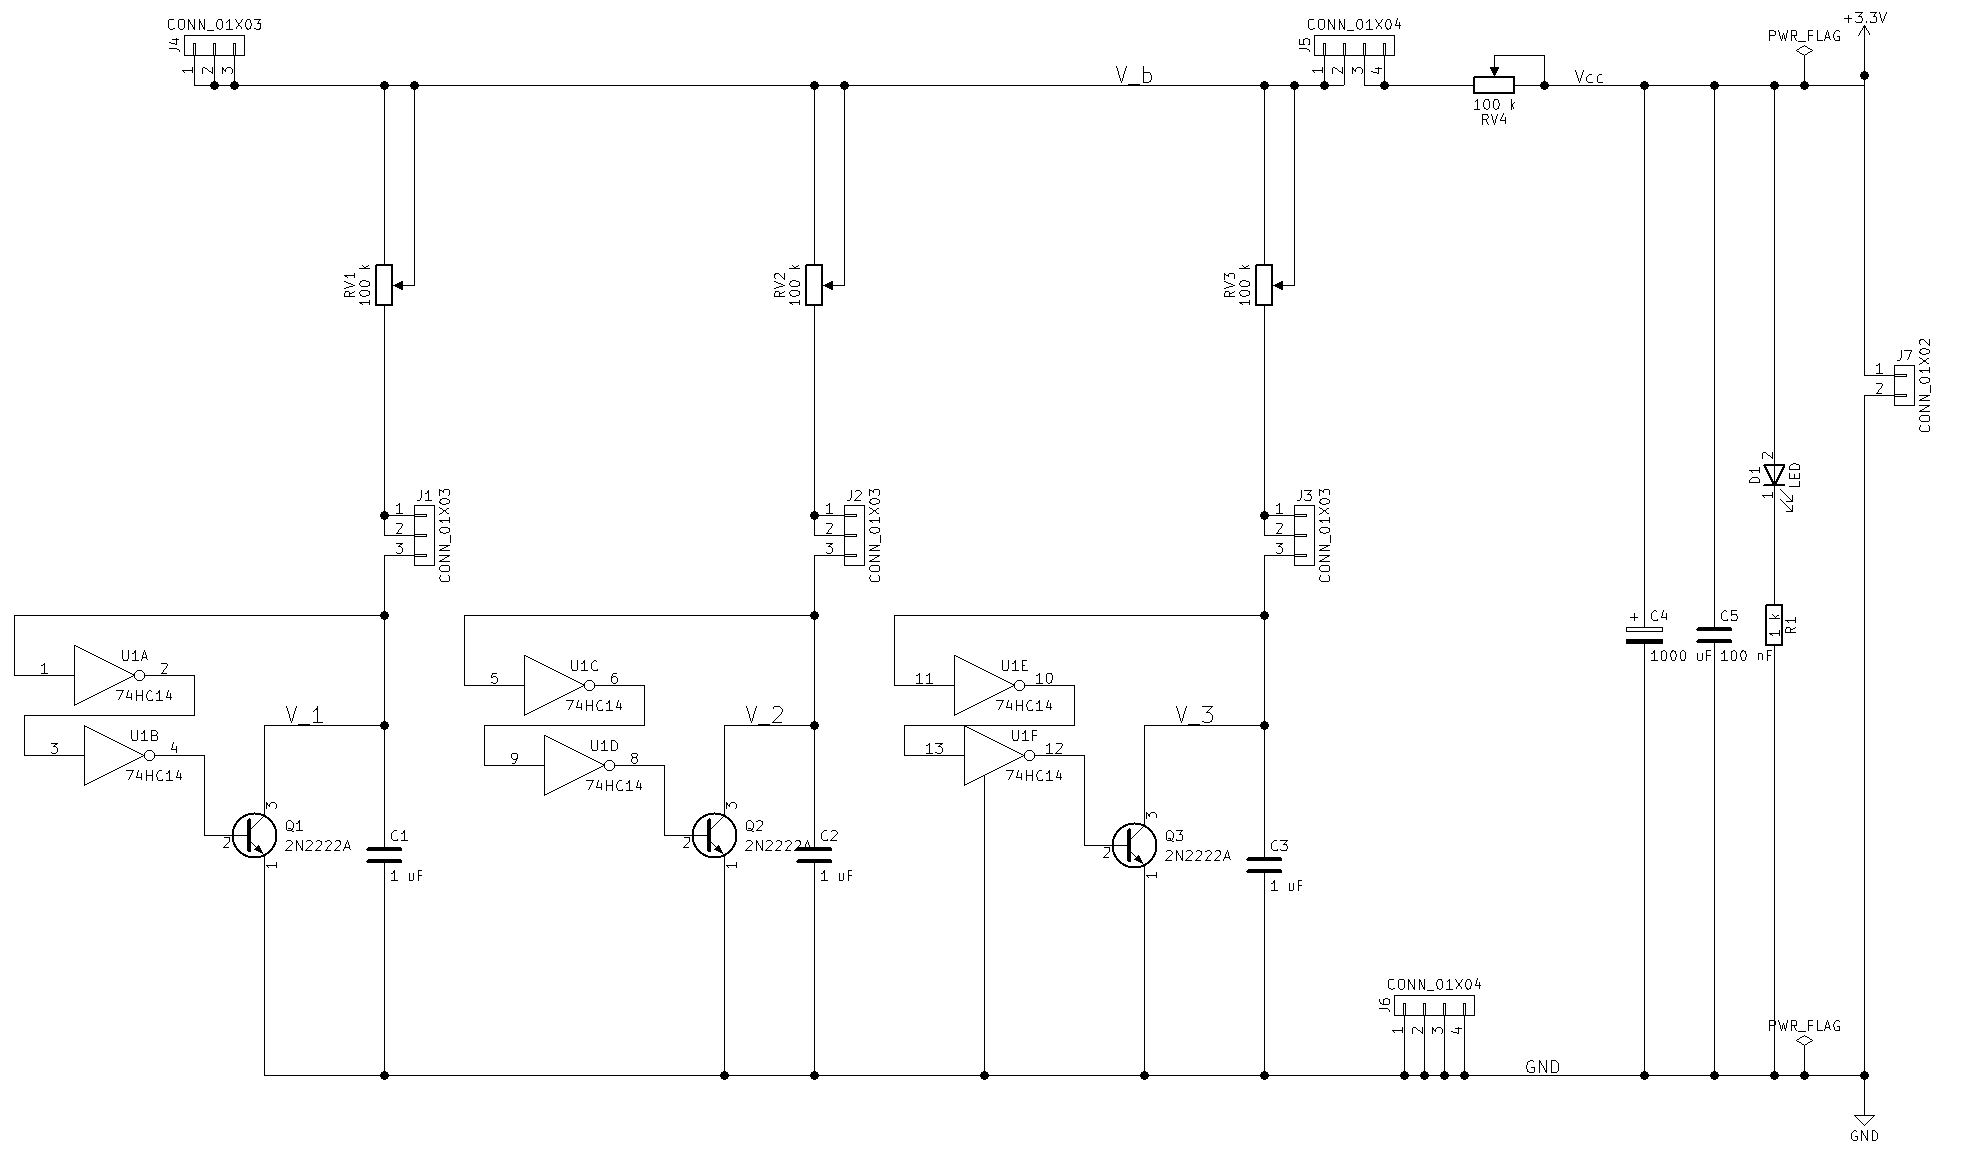
\includegraphics[width=0.7\textwidth]{p/relax3ds_schem.png} }
  \caption{Электрическая схема системы из трёх связанных релаксационных генераторов на основе триггеров Шмидта}
  \label{atu:relax3ds_schem}
\end{figure}


Динамика.

\section{Модели систем из трёх связанных релаксационных генераторов}


\section{Критерии идентификации систем из трёх связанных релаксационных генераторов}

\section{Идентификация параметра системы из трёх связанных релаксационных генераторов}

\section{Выводы по разделу \thechapter}

Выводы.

